\documentclass[11pt]{article}

%use European style
\usepackage[a4paper,left=2cm,right=2cm,top=2cm,bottom=2cm]{geometry}

%few useful packages ------------------------------------------------------------------
	\usepackage{setspace}
		\let\Tiny=\tiny %remove annoying warnings
	\usepackage[english]{babel}
	\usepackage[latin1]{inputenc}
	\usepackage{amsfonts}
	\usepackage{amsmath}
	\usepackage{amssymb}
	\usepackage{amsthm}
	\usepackage{amsfonts}
	\usepackage{colortbl}
	\usepackage{float}
	\usepackage{xcolor}
	\usepackage{eurosym}
	\usepackage{enumitem}
	\usepackage{chngpage}
	\usepackage{fancyhdr}
	\usepackage{fancyvrb}
	\usepackage{float}
	\usepackage{framed}
	\usepackage{multirow}
	\usepackage{physics}
	\usepackage{graphicx}
		\graphicspath{ {./images/} }
	\usepackage{geometry}
	\usepackage{lipsum}
	\usepackage{tabularx}
	\usepackage{url}
	\usepackage[linktocpage]{hyperref}
	
	%define environment for code
	\definecolor{orangepse}{RGB}{240,139,39}
	\definecolor{redpse}{RGB}{222,6,61}
	\newcommand{\rpse}[1]{\textcolor{redpse}{#1}}
	\definecolor{dkgreen}{rgb}{0,0.6,0}
	\definecolor{gray}{rgb}{0.5,0.5,0.5}
	\definecolor{mauve}{rgb}{0.58,0,0.82}
	
	\usepackage{listings}
			\lstset{frame=tblr,
				language=R,
				aboveskip=5mm,
				belowskip=5mm,
				showstringspaces=false,
				columns=flexible,
				basicstyle={\small\ttfamily},
				numbers=none,
				numberstyle=\tiny\color{gray},
				keywordstyle=\color{blue},
				commentstyle=\color{dkgreen},
				stringstyle=\color{mauve},
				breaklines=true,
				breakatwhitespace=true,
				tabsize=3
			}
%---------------------------------------------------------------------------------------
\usepackage[backend=biber, style=authoryear, maxcitenames=3, citestyle=apa]{biblatex}

\addbibresource{bib.bib} 

% New Commands ----------------------------
\newcommand{\bb}{\bigbreak\noindent}
\newcommand{\mycomment}[1]{}

%----------------------------------------------------------

\definecolor{titlepagecolor}{cmyk}{1,.60,0,.40}
\definecolor{namecolor}{cmyk}{1,.50,0,.10} 

% Preamble information:
%%%%%%%%%%%%%%%%%%%%%%%%%%%%%%%%%%%%%%%%

\title{INSERT TITLE}
\author{Davide Davies-Biletta  }


%%%%%%%%%%%%%%%%%%%%%%%%%%%%%%%%%%%%%%%%


\begin{document}
\begin{spacing}{2}

\thispagestyle{empty}
\begin{center}
	
	
	\begin{minipage}{0.55\textwidth}
		\centering
		
\includegraphics[width=1\linewidth]{"images/Pantheon Sorbonne Logo.png"}
	\end{minipage}%
	\begin{minipage}{0.5\textwidth}
		\centering
		\includegraphics[width=0.35\linewidth]{"images/PSE_logo"}
	\end{minipage}
		
	
	\begin{minipage}{0.85\linewidth}
		\centering
		\vspace{1cm}
		{{\Large{ \textbf{Cognitive Discounting in the Case of 
				Distortionary Taxes}} \\
		 \Large{Implications for Fiscal Policy and Deficit Dynamics} \par}}
			
			
		\vspace{3cm}
		%Author's name
		{\Large Davide Davies-Biletta\par}
		{\large Supervised by Tobias Broer\par}
		
		\vspace{4cm}
		{\Large A thesis submitted for the degree of\\
			 M2 Analysis \& Policy in Economics\par}
		\vspace{2cm}
		%Date
		{\Large August 2023}
	\end{minipage}
\end{center}
\clearpage
\pagenumbering{roman}
\begin{center}
	\begin{minipage}{0.90\linewidth}
		\centering
		\vspace{3cm}
		{\Large \textbf{Acknowledgements}\par}
		\vspace*{10pt}
		I would like to express my gratitude to my supervisor, Tobias Broer, for his patience in indulging my particular fascination with this topic, even at times when I felt adrift.
		\bb
		I also extend my sincerest thanks to Olivier Blanchard for his invaluable insights and for generously dedicating time to numerous meetings, to which I often arrived with very little and left with a wealth of knowledge.
		\bb
		Special thanks also are due to Paul De Grauwe, whose guidance and encouragement set me on the path to behavioural macroeconomics. His work not only opened my eyes to this field, but our conversations and correspondence played a crucial role in my decision to pursue this master's program, helping me to bridge the gaps in my understanding.
		\bb
		Je voudrais �galement remercier Daniel, Habib, et Claire, qui m'ont permis de me sentir chez moi � Paris tout au long de mon s�jour et qui m'ont offert une famille lorsque la mienne n'�tait pas proche.
		\bb
		Finally, I would also like to extend my appreciation to my Mother, my Father, and the Coinage brothers. Without their love and support, none of this would have been possible.
	\end{minipage}
\end{center}
\clearpage

\begin{center}
\begin{minipage}{0.80\linewidth}
	\vspace{3cm}
\begin{center}
	{\Large \textbf{Abstract}\par}
\end{center}
\bb
This paper extends the Behavioural New Keynesian model by incorporating distortionary taxes and analysing their effects through the lens of cognitive discounting. We begin by developing and examining a framework with distortionary taxes but without deficit spending, evaluating the robustness of fiscal policies under cognitive discounting. We then investigate how incorporating deficit spending modifies these dynamics, focusing on debt sustainability and fiscal multipliers. Our results highlight that behavioural biases influence fiscal policy outcomes in significant ways, leading to higher fiscal multipliers compared to traditional models. This extension enriches our understanding of the interaction between Behavioural biases and fiscal policy, offering valuable insights for both theoretical research and practical policy formulation.
\vspace{1cm}
\begin{center}
	JEL: E7, E70, E12, E6, E62, E40, E63, H20
\end{center}

\end{minipage}
\end{center}
\pagebreak
\tableofcontents

\pagebreak
\pagenumbering{arabic}





\section{Introduction}
The intersection of behavioural economics and macroeconomics has witnessed a burgeoning interest in recent years, as researchers seek to bridge the gap between theoretical models and empirical observations. Traditional macroeconomic models, and a vast portion of policy analysis still rely heavily on rational expectations models, often with perfectly rational, forward-looking representative agents \parencite{hommes2021behavioural}. Such an assumption is quite stringent because it requires agents to have complete knowledge of all potential future states and to be able to create fully state-contingent plans by solving intricate optimization problems. However, numerous empirical studies using survey data tend to reject the idea of full information rational expectations \parencite{coibion2015information,bordalo2020overreaction}. In response, there has been an emergence of a behavioural macroeconomic field of research, which aims to challenge these strict assumptions of rationality, claiming to better capture more nuanced, real-world economic behaviour.
\bb
One notable  advancement in the field has been the work done by Xavier Gabaix on sparse maximization \parencite{gabaix2014sparsity,gabaix2016behavioural}, which provides a tractable approach to modelling bounded rationality and cognitive limitations within macroeconomic frameworks. Building on this foundation, \cite{gabaix2020behavioural} introduced a behavioural extension of the New Keynesian model. This model incorporated elements of bounded rationality into the traditional framework, enhancing our understanding of both monetary and fiscal under cognitive constraints. However, the extent of Gabaix's analysis of fiscal policy, within the Behavioural New Keynesian (BeNK) model, is restricted solely to the use of lump-sum taxes. While this approach has laid crucial groundwork for behavioural macroeconomic research, it does not address the complexities introduced by more realistic taxes policies. 
\bb
Our paper aims to extend the current Behavioural New Keynesian framework by integrating distortionary taxes, such as those on labour and consumption. This extension seeks to deepen our understanding of how fiscal decisions influence economic behaviour within a behavioural context. To achieve this, we first incorporate cognitive constraints into an existing New Keynesian model that already includes distortionary taxes. Our approach draws on foundational insights from seminal works by \cite{correia2013unconventional} and \cite{eggertsson2011fiscal}. Both papers investigate the impact of fiscal policy during periods of economic slack, highlighting the crucial role of distortionary taxes in determining the effectiveness of fiscal interventions. Yet, while \cite{eggertsson2011fiscal} focuses on the effects of altering one tax at a time, \cite{correia2013unconventional} examines the simultaneous adjustment of multiple taxes. By incorporating there model into a behavioural framework, our aim is to evaluate how cognitive biases and bounded rationality influence the robustness of their findings.
\bb
Our work is therefore closely aligned with recent contributions by \cite{bianchi2024fiscal}, who examined the sensitivity of fiscal policy, as outline in \cite{correia2013unconventional}, to the rational expectations assumption. Building on \cite{farhi2019monetary}, Bianchi employs a level-\textit{k} thinking model that incorporates bounded rationality by accounting for varying degrees of cognitive sophistication among agents. Their findings suggest that the effectiveness of distortionary taxes remains robust even when deviating from the rational expectations paradigm. Similarly, our research, which utilizes a cognitive discounting model, corroborates these results, demonstrating that the efficacy of distortionary taxes is consistent under alternative assumptions about cognitive constraints.
\bb
In the second part of our paper, we examine how distortionary taxes influence deficit dynamics within a behavioural framework. Traditional New Keynesian models, which assume Ricardian equivalence, suggest that government financing methods?whether through taxes or debt?do not affect overall economic activity since rational agents adjust their savings to offset future tax liabilities. However, \cite{gabaix2020behavioural} and \cite{woodford2019policy} show that bounded rationality can disrupt Ricardian equivalence, causing significant impacts on aggregate demand and economic activity. Behavioural agents, in particular, perceive government debt as an increase in their wealth, leading to higher consumption and altered economic dynamics. To explore these effects, we incorporate the deficit dynamics proposed by \cite{uhlig2010some} into our behavioural New Keynesian framework. Unlike \cite{gabaix2020behavioural} and \cite{woodford2019policy}, which analyse only lump-sum taxes, our model includes distortionary taxes. This approach allows us to assess how the structure of deficit financing and the associated tax distortions influence the dynamics of government debt and the fiscal multiplier. Our findings are consistent with previous those of other behavioural frameworks however the dynamics differ slightly. 
\bb
Ultimately, our analysis provides a foundation for future research into the broader implications of cognitive discounting in macroeconomic modelling. The results from our representative agent model serve as a foundation for future extensions such as the inclusion of distortionary taxes in heterogeneous agent models,  such as the one developed by  \cite{pfauti2022behavioural}, and the investigation of progressive taxation, such as \cite{ferriere2024heterogeneous}, within a behavioural context. These extensions could provide further insights into the distributional effects of fiscal policy under cognitive discounting and deepen our understanding of the macroeconomic implications of behavioural biases.
\bb
This research should be of interest not only to academics but also to policymakers. By highlighting how cognitive constraints and distortionary taxes influence economic dynamics, our findings can inform more effective and realistic fiscal policies. Understanding these effects is crucial for designing interventions that align with actual economic behaviour, thereby improving the efficacy of policy measures in real-world scenarios.



\subsection{Outline}
This paper begins by introducing traditional New Keynesian model with distortionary taxes as developed in papers by \cite{correia2013unconventional} and \cite{correia2013unconventional}. This will serve as a foundation on which we can build and provides a basis for understanding how distortionary taxes, such as those on labour and consumption, influence economic behaviour under standard assumptions.
\bb
The analysis then shifts to incorporate these distortionary taxes into a Behavioural New Keynesian framework, building on the bounded rationality model proposed by \cite{gabaix2014sparsity}. We first explain the concept of cognitive discounting, where individuals place greater emphasis on present conditions over future outcomes, and demonstrate how this cognitive bias can be operationalized within our economic model.
\bb
We round out the first part of the analysis by examining the sensitivity of fiscal policy outcomes to the presence of cognitive discounting. Specifically, it investigates how the behavioural biases affect the standard trade-offs associated with distortionary taxes, such as the impact on labour supply, and consumption decisions. This section builds on the previous literature by adapting their insights and comparing their results with those from a behavioural context. This section aims to provide more nuanced understanding of how these taxes function in a world where agents do not possess perfect foresight.
\bb
In the second part, the paper extends the analysis to consider the role of deficit financing within this adapted behavioural framework. We look to integrate these new distortionary taxes into the modelling of debt dynamics. Drawing on previous work by \cite{uhlig2010some} this thesis incorporates a model of debt dynamics following a government spending shock. Here, the analysis focuses on how the interaction between cognitive discounting and deficit financing alters the traditional conclusions drawn from models that assume rational expectations. Specifically, it explores how different degrees of deficit financing, ranging from scenarios where government spending is fully financed by taxes to those where it is primarily financed by debt, affect the overall economic multipliers.
\bb
This research makes several key contributions to the literature. First, by introducing cognitive discounting into a model with distortionary taxes, it provides new insights into the effectiveness of fiscal policy in a more realistic setting where agents exhibit bounded rationality. Second, the inclusion of deficit financing within this behavioural framework offers a novel perspective on how debt dynamics and fiscal sustainability are influenced by cognitive limitations.
\bb
This paper thus seeks to advance our understanding of fiscal policy in the presence of behavioural biases, offering theoretical and practical insights that could inform both academic research and policymaking. The findings are particularly relevant in a contemporary context where governments frequently resort to deficit spending, and where the behavioural responses of economic agents can have profound implications for the success or failure of fiscal interventions.




\section{The Standard Model}
This section summarizes a standard New Keynesian DGSE model as seen in \cite{correia2013unconventional} and \cite{eggertsson2011fiscal}.
At its core, this is a standard stochastic growth model (real business cycle model) with two added frictions: a monopolistic competition among firms and frictions in the firms' price setting through fixed nominal contracts that have a stochastic duration as in \cite{calvo1983staggered}. This model however, has a more detailed description of taxes. This section summarizes a simplified version of the model that will serve as the baseline illustration. Those familiar with the paper and its derivations may find it more useful to skip directly to the proceeding sections in which we introduce the notion of behavioural agents.
\bb
The model contains three types of agents, a representative household, a continuum of monopolistic firms, and a set of policymakers, made up of a central bank and a fiscal authority. The optimization problem of the household results in an output Euler-equation, interchangeably refereed to as the IS-curve, the firms' problem results in a Phillips-curve governing inflation dynamics, and the model is closed by specifying the behaviour of the policy authorities in terms of feedback rules.

\subsection{Households}
The household maximizes the inter-temporal utility function:
\begin{align}
	U_t = \mathbb{E}_t \sum_{t=0}^{\infty} \beta^t \xi_t \left( \frac{C_t^{1-\sigma}}{1-\sigma} - \frac{N_t^{1+\varphi}}{1+\varphi} \right)
\end{align}
subject to the budget constraint:
\begin{align}
	P_t(1+\tau_t^c)C_t + B_t = R_{t-1}B_{t-1} + (1 - \tau_t^n)W_t N_t + (1 - \tau_t^d)\Pi_t + T_t
\end{align}
where \( C_t \) denotes consumption, \( N_t \) represents employment with the nominal wage \( W_t \), \( B_t \) is a risk-free nominal government bond paying a gross nominal interest rate \( R_t \) (with \( R_t = 1+i_t \)), \( T_t \) is a lump-sum tax, and \( P_t \) is the aggregate price level. The household is also the residual claimant of firms' aggregate profits \( \Pi_t \). The parameters \( 0 < \beta < 1 \) is the discount factor, \( \sigma > 0 \) is the coefficient of relative risk aversion, and \( \varphi > 0 \) represents the labour supply elasticity. \( \mathbb{E}_t \) denotes the standard rational expectations operator. Taxes on consumption, labour, and profits are denoted by \( \tau_t^c \), \( \tau_t^n \), and \( \tau_t^d \), respectively. As in \cite{correia2013unconventional}, we assume that profits are fully taxed, implying \( \tau_t^d = 1 \).
\bb
From the first-order conditions, we derive the consumption Euler equation:
\begin{align}
	\frac{u_C(C_t, N_t)\xi_t}{P_t(1+\tau_t^c)} &= \beta R_t \mathbb{E}_t \frac{u_C(C_{t+1}, N_{t+1}) \xi_{t+1}}{P_{t+1}(1+\tau_{t+1}^c)} \\
	u_C(C_t, N_t) &= \beta R_t \mathbb{E}_t u_C(C_{t+1}, N_{t+1}) \frac{\xi_{t+1}}{\xi_t} \frac{P_t}{P_{t+1}} \frac{(1+\tau_t^c)}{(1+\tau_{t+1}^c)}.
\end{align}
This equation illustrates the influence of the ex-ante real interest rate, given by \( R_t \mathbb{E}_t \pi_{t+1}^{-1} \), on the inter-temporal allocation of consumption between periods \( t \) and \( t+1 \). Additionally, it highlights the crucial role of changes in consumption taxes. Additionally, the labour supply condition is derived as:
\begin{align}
	- \frac{U_N(C_t, N_t)}{U_C(C_t, N_t)} &= \frac{(1-\tau_t^n)W_t}{(1+\tau_t^c)P_t}
\end{align}
which reflect the first-order conditions of the household's utility maximization problem.
\bb
Ultimately, we can express the Euler equation in log-linear terms:
\begin{align}
	\hat{C}_t &= \mathbb{E}_t \hat{C}_{t+1} - \frac{1}{\sigma} \mathbb{E}_t (\hat{i}_t - \hat{\pi}_{t+1} - r_t) + \frac{1}{\sigma} \mathbb{E}_t (\hat{\tau}_{t+1}^c - \hat{\tau}_t^c)
\end{align}
where \( r_t \) represents the real interest rate, and each variable with a hat above it denotes its log-deviation from the non-stochastic steady state.


\subsection{Firms}
Firms are assumed to follow a production function given by:
\begin{align}
	Y_t = A_t N_t^\alpha
\end{align}
where \( Y_t \) denotes output, and \( A_t \) represents an exogenous productivity shock.
\bb
Firms operate in a monopolistically competitive market and possess pricing power over their final output. Final goods are imperfectly substitutable among an infinite set of varieties indexed by \( i \in [0, 1] \). Each \( i \)-th variety is produced by a distinct firm and aggregated via the CES Dixit-Stiglitz aggregator:
\begin{align}
	C_t = \left[ \int_0^1 C_t(i)^{\frac{\varepsilon-1}{\varepsilon}} \, di \right]^{\frac{\varepsilon}{\varepsilon-1}}
\end{align}
where \( \varepsilon > 1 \) is the elasticity of substitution among different final goods varieties. The demand function for variety \( i \) is:
\begin{align}
	Y_t(i) = \left[ \frac{p_t(i)}{P_t} \right]^{-\varepsilon} Y_t
\end{align}
where \( p_t(i) \) is the price of the \( i \)-th variety, \( Y_t \) is aggregate demand, and
\begin{align}
	P_t = \left[\int_0^1 p_t(i)^{1-\varepsilon} \, di \right]^{\frac{1}{1-\varepsilon}}
\end{align}
is the aggregate price index.
\bb
Under Calvo-type price setting, firms can reset their prices with probability \( 1 - \theta \), while with probability \( \theta \), they keep their price fixed. A rational firm's optimal pricing problem is to maximize profits, given by:
\begin{align}
	\max \mathbb{E}_t \sum_{k=0}^{\infty} (\theta \beta)^k \lambda_{t+k} \left[ P_{t+k}Y_{t+k} - W_{t+k}Y_{t+k} \right]
\end{align}
where \( \lambda_{t+k} \) is the marginal utility of nominal income for the representative household. An important assumption from \cite{eggertsson2011fiscal} is that the price set by the firm excludes sales tax. Thus, a reduction in sales taxes directly lowers the consumer price by the amount of the tax cut for firms that have not yet reset their prices.
Using the assumption that a fraction \( \theta \) of firms keep their prices fixed while \( 1 - \theta \) reset them to \( p_t \), we can express the price index as:
\begin{align}
	P_t = \left[ (1- \theta)(p_t)^{1-\varepsilon} + \theta P_{t-1}^{1-\varepsilon} \right]^{\frac{1}{1-\varepsilon}}
\end{align}
\bb
Following the standard derivation for Calvo pricing, \cite{correia2013unconventional} derives the Behavioural Phillips curve:
\begin{align*}
	\pi_t &\approx \beta \mathbb{E}_t \pi_{t+1} + \kappa \hat{y}_t + \kappa \psi (\hat{\tau}_t^c + \hat{\tau}_t^n)
\end{align*}
This formulation differs slightly from the Phillips curve presented in \cite{eggertsson2011fiscal}, as \cite{correia2013unconventional} assumes that government spending \( G_t = G \).


\subsection{Taylor Rule}
Both \cite{eggertsson2011fiscal} and \cite{correia2013unconventional} assume passive monetary policy which explicitly accounts for the lower bound on nominal interest rates. Such that the nominal interest rate must always be equal to or lager than 0. 
\begin{align*}
	i_t \geq 0
\end{align*}
Central banks in our model therefore follow a Taylor rule in accordance with: 
\begin{align}
	\hat{i}_t = \max \{ \: 0, \: r_t^n + \phi_\pi \pi_t + \phi_y \hat{y}_t \: \} 
\end{align}

\subsection{Government}
The government aims to minimize expenditure on individual goods for a given level of aggregate spending. To finance this expenditure, it utilizes time-varying taxes on consumption, \( \tau_t^c \), and labor income, \( \tau_t^n \). Additionally, lump-sum taxes, \( T_t \), are employed as a residual variable to ensure the government budget constraint is met. 
\bb
Given the aggregate price index:
\begin{align}
	P_t = \left(\int_0^1 p_{it}^{1-\epsilon} \, di \right)^{\frac{1}{1-\epsilon}},
\end{align}
where \( p_{it} \) represents the price of variety \( i \), the minimization of expenditure on individual goods implies that the share of expenditure on variety \( i \) is given by:
\begin{align}
	\frac{g_{it}}{G_t} = \left(\frac{p_{it}}{P_t}\right)^{-\epsilon}.
\end{align}
While \cite{correia2013unconventional} assumes constant government spending, their framework allows for a set of policy variables that can be adjusted in response to economic shocks. This flexibility makes fiscal policy a powerful tool for managing economic fluctuations.


\subsection{Calibrating Fiscal Policy to Avoid a Recession}
Let us now look to how we might adjust fiscal policy in response to such a shock. Consider a particular case, outlined in both \cite{eggertsson2011fiscal} and \cite{christiano2011government}  in which a negative preference shock, in combination with the meeting of the zero lower bound condition, generates a potentially large recession. For the sake of simplicity, as in  \cite{correia2013unconventional}, we assume that $G_t = G$, $A_t = 1$, so that the only shock is the preference shock. These strict assumptions imply that the efficient allocation is constant and unaffected by preference shock. Importantly, we notice from our utility function that preferences ($\xi_t$) are multiplicative. 
\begin{align}
	u(C_t, N_t, \xi_t) = u(C_t, N_t)\xi_t
\end{align}
In this way, the preference shock does not affect the marginal rate of substitution between consumption and leisure. It will, however, affect an agents inter-temporal consumption choice between time $t$ and time $t + 1$. 
Hence, both \cite{eggertsson2011fiscal} and \cite{christiano2011government} consider a case in which $\xi_t$ evolves exogenously according to: 
\begin{align*}
	\dfrac{\xi_t}{\xi_{t+1}} \: &< \: \beta \text{  for  } t = 0,1,2, \dots,T-1\\
	\dfrac{\xi_t}{\xi_{t+1}} \: &= \: 1 \text{  for  } t = T,T+1,T+2, \dots
\end{align*} 
This results in a natural rate of interest given by \(\frac{\xi_t}{\xi_{t+1}} < 1\) if \(t < T\) and \(\frac{\xi_t}{\xi_{t+1}} > 1\) for \(t \geq T\). We set the nominal interest rate to \(1 + i_t = 1\) for \(t \leq T - 1\) and \(1 + i_t = \frac{1}{\xi}\) for \(t > T\). \cite{correia2013unconventional} sets the path of consumption taxes according to
\[
\frac{1 + \tau_{t+1}^c}{1 + \tau_t^c} = \beta\frac{\xi_{t+1}}{\xi_t}, \quad \text{for } t = 0, 1, 2, \dots, T - 1.
\]
And sets labour taxes as follows:
\[
\dfrac{(1 + \tau_t^c)}{(1 - \tau_t^n)} \frac{\epsilon}{\epsilon - 1} = 1, \quad \text{for all } t.
\]
\bb
In this deterministic model, the initial level of the consumption tax \(\tau_0^c\) determines the future paths of both consumption and labour taxes. Consumption taxes rise over time until they stabilize, while labour taxes decrease and then stabilize. The strategy aims to induce inflation in consumer prices while keeping producer prices stable, leading to negative real interest rates and avoiding distortions from producer price inflation. To achieve this, a temporary reduction in consumption tax must be paired with a temporary increase in labour tax to counteract the lowered marginal cost for firms and prevent them from reducing prices. 
\bb
\begin{figure} [h!]
	\centering
	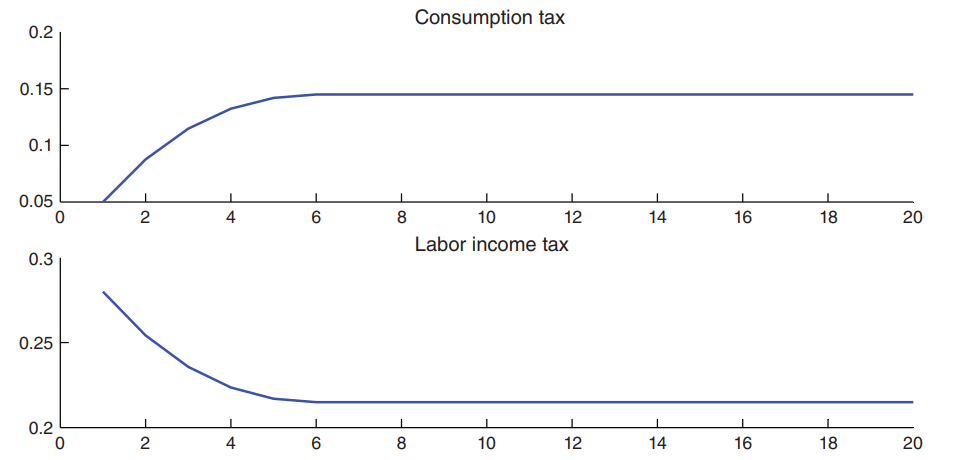
\includegraphics[width=0.7\linewidth]{images/correia2013}
	\caption{Dynamic Path for Unconventional Taxes, Sticky Prices, Flexible Wages}
	\small{Time, measured in quarters, is on the horizontal axis. Taxes are measured in levels}
	\label{fig:correia2013}
\end{figure}
\bb
Thus, \cite{correia2013unconventional} find that when facing a preference shock, there exists a path for both labour and consumption taxes that ensures a smooth transition back to the steady state. This approach carefully balances the adjustments in taxes to manage inflationary pressures without causing significant disruptions to the economy. The dynamic path illustrated in Figure \ref{fig:correia2013} demonstrates how these tax adjustments unfold over time, showing a gradual return to equilibrium.



\section{The Behavioural Model}
We now look to introduce behavioural aspects into what is currently a more traditional New Keynesian model consisting solely of perfectly rational agents. The ensuing Behavioural New Keynesian model retains the same structural elements as the standard model: inter-temporal household decisions are governed by an Euler-equation, firms' pricing decisions are represented by a Phillips-curve, and monetary and fiscal policies are implemented via feedback rules. However, unlike the standard model, expectations are not fully rational. Instead, they reflect behavioural adjustments due to agents' cognitive limitations, particularly in their perception of future events.

\bb In this framework, agents simulate the future but do so with cognitive discounting, shrinking their simulations toward a simple benchmark, the steady state of the economy. This follows from the idea that agents receive noisy signals about the state of the economy, which makes them less confident about distant future events. Consequently, an innovation that is expected to occur in $k$ periods is perceived with diminished significance, discounted by a factor $\bar{m}^k$ relative to the rational response, where $\bar{m}\in [0,1] $ is a parameter capturing the degree of cognitive discounting. This means that innovations far in the future are heavily discounted compared to the rational benchmark, which corresponds to the case where $\bar{m} = 1$. In essence, the agent remains globally patient with respect to steady-state variables but exhibits myopia regarding deviations around the steady state, particularly those that are expected to occur in the distant future.

\subsection{General Approach}
Behavioural macroeconomics attempts to incorporate the idea that expectation formation is not necessarily based on perfect knowledge about the future evolution of all economically relevant variables \parencite{woodford2013macroeconomic}. Instead of possessing perfectly accurate forecasts, agents in this model may hold perceptions of reality that are imprecise and not entirely forward-looking. Under rational expectations, agents are assumed to have complete and perfect knowledge about the potential future paths of all variables. However, in practice, there are likely to be variables for which forming such precise expectations is challenging. This can be modelled as agents discounting the information that would otherwise be fully utilized by a rational agent. Various behavioural models incorporate this feature, including those with rationally inattentive agents, agents engaged in signal extraction, or those employing simple learning mechanisms. As a result, cognitive discounting leads to decision rules that, while appearing similar to those in standard rational expectations models, are adjusted to account for the behavioural deviations from full rationality.
\bb
In order to make a behavioural macroeconomic model internally consistent, two key elements are needed. First, an expectation formation mechanism that is consistent with the informational structure of the model economy, while boundedly rational. More specifically, the resulting deviations from fully rational expectations are not ad hoc but are subject to internal discipline and consistency. \cite{gabaix2014sparsity, gabaix2016behavioural} show how to derive an appropriate expectations operator via the concept of sparse dynamic programming. Second, a researcher still has to make assumptions on the agents' information set, or specifically, what economically relevant information the agents perceive. Looking at \cite{lubik2021fiscal}, we can see a concise summary of this on which I will expand.

\bb
Consider a state variable $\boldsymbol{X}_t$ (comprising productivity $A_t$, preference shocks $\zeta_t$, as well as announced actions in monetary and fiscal policy), that will evolve in equilibrium as:
\begin{align}
	\boldsymbol{X}_{t+1} = \boldsymbol{G^X}(\boldsymbol{X}_t, \boldsymbol{\epsilon}_{t+1})
\end{align} 
for some equilibrium transition function $\boldsymbol{G^X}$ and mean-0 innovations $\boldsymbol{\epsilon}_{t+1}$ (which depend on the equilibrium policies of the agent and the government). If we assume that $\boldsymbol{X}_t$ has a mean 0 and linearise, we get:
\begin{align}
	\boldsymbol{X}_{t+1} = \boldsymbol{\Gamma X}_t + \boldsymbol{\epsilon}_{t+1}
\end{align}
where $\boldsymbol{\Gamma}$ is a matrix of coefficients and the vector $\boldsymbol{\epsilon}_{t+1}$ represents innovations to the dynamic system which are typically assumed to have zero mean and are \textit{i.i.d}. This equation therefore captures all the information that is potentially available to the agent. 
\bb
In our behavioural environment however, we assume that agents can be cognitively limited and thus perceive a modified version of the equation in which they do not fully perceive future changes in state variables. Hence we modify the equation to account for this:
\begin{align}
	\boldsymbol{X}_{t+1} = M\boldsymbol{G^X}(\boldsymbol{X}_t, \boldsymbol{\epsilon}_{t+1}) = M(\boldsymbol{\Gamma X}_t + \boldsymbol{\epsilon}_{t+1})
\end{align}
where M is a matrix containing corresponding cognitive discounting parameters. Each of these parameters take a value between 0 and 1. In the case the rational agent, they perfectly perceive the future path of each state variable, hence they are characterised by a parameter value of 1. Behavioural agents on the other hand, do not and so are characterised by parameter values below 1. 
Under expectation, the innovations disappear. The expectation of a cognitively limited agent is thus $ \mathbb{E}_t^{BR} \boldsymbol{X}_{t+1} = M\boldsymbol{\Gamma X}_t $ while that of the rational agent is simply:  $\mathbb{E}_t \boldsymbol{X}_{t+1} = \boldsymbol{\Gamma X}_t $. Therefore:
\begin{align}
	\label{eq:lemma}
	 \mathbb{E}_t^{BR} \boldsymbol{X}_{t+1} = M \:\mathbb{E}_t \boldsymbol{X}_{t+1}
\end{align}
Iterating over time, we can see that:
\begin{align}
	\mathbb{E}_t^{BR} \boldsymbol{X}_{t+k} = M^k \:\mathbb{E}_t \boldsymbol{X}_{t+k}
\end{align}
Recalling that each of the parameters within $M$ are contained between 0 and 1, we see that the more distant the events in the future, the more the behavioural agent ``sees them dimly", i.e. sees them with a dampened cognitive discount factor $M^k$ at horizon $k$. In light of this, behavioural macroeconomics results in the idea of a ``discounted Euler-equation.''

\subsection{The Behavioural Euler Equation}
In a standard New Keynesian framework, the Euler equation governs the time path of output by linking it to the real interest rate and aggregate shocks, reflecting the inter temporal consumption-savings choices made by households. The Behavioural Euler Equation shares the same foundational structure, but it incorporates a critical departure from the traditional model by assuming that agents do not fully observe or process all available information. Instead, they focus on a subset of key economic variables, leading to a more simplified and cognitively constrained decision-making process.
\bb
Building on the earlier discussion of cognitive discounting, where agents' expectations about future variables are attenuated by the matrix \( M \) (as shown in Equation \ref{eq:lemma}), this adjustment carries over to the Euler equation. In the behavioural framework, the agents' perception of future consumption, prices, and taxes is not perfectly aligned with the actual expected values. Instead, these perceptions are "discounted" according to the attention parameters, which reflect the degree of imperfect cognition.
\bb
This leads to a modified version of the Euler equation where the marginal utility of consumption today, denoted as \( u_C(C_t, N_t) \), is related to the expected discounted utility of future consumption, \( \mathbb{E}_t^{BR} u_C(C_{t+1}, N_{t+1}) \), adjusted for the nominal interest rate \( 1+i \), the ratio of preference shocks \( \frac{\xi_{t+1}}{\xi_t} \), the ratio of current to future prices \( \frac{P_t}{P_{t+1}} \), and the relative consumption tax adjustments \( \frac{(1+\tau_t^c)}{(1+\tau_{t+1}^c)} \). The Behavioural Euler Equation is expressed as:

\begin{align}
	\label{eq: inter-temporal_BR}
		u_C(C_t, N_t) =& (1+i) \beta \mathbb{E}_t^{BR} u_C(C_{t+1}, N_{t+1}) \dfrac{\xi_{t+1}}{\xi_t}\dfrac{P_t}{P_{t+1}} \dfrac{(1+\tau_{t}^c)}{(1+\tau_{t+1}^c)}.
\end{align}
\bb
If we log-linearize equation \ref{eq: inter-temporal_BR}, we obtain:
\begin{equation*}
	\delta \hat{C}_t + \Gamma \hat{\xi}_t - \hat{\tau}^c_t =  \left[\hat{i}_t - \ln\left(\frac{1}{\beta}\right) - \mathbb{E}_t \pi_{t+1}\right] + \mathbb{E}_t^{BR} \left[\delta \hat{C}_{t+1} + \Gamma\hat{\xi}_{t+1} - \hat{\tau}^c_{t+1}\right]
\end{equation*}
where $\delta = \dfrac{C }{u_c}(u_{CC }+ u_{CN })$, and $\hat{C}_t = \ln\left(\frac{C_t}{C}\right)$,  $\hat{\tau}^c_t = \ln\left(\frac{1+\tau^c_t}{1+\tau^c}\right)$, and $\pi_{t+1} = \ln\left(\frac{P_{t+1}}{P_t}\right)$.  Notice, that  the expectation term in front of inflation $\mathbb{E}_t \pi_{t+1}$, in the IS-curve remains unaffected and does not incorporate any behavioural biases. This is because our model does not contain the concept of nominal illusion. One could include it as outlined in a footnote by \cite{gabaix2020behavioural}, yet for simplicity we do not. 
Furthermore,  we know that because $\xi$ is multiplicative, deviations between periods effects consumption proportionally, hence we can say $\Gamma = 1$ and rewrite the equation as follows;

\begin{equation*}
	\delta \hat{C}_t +  \hat{\xi}_t - \hat{\tau}^c_t =  \left[\hat{i}_t - \ln\left(\frac{1}{\beta}\right) - \mathbb{E}_t \pi_{t+1}\right] + \mathbb{E}_t^{BR} \left[\delta \hat{C}_{t+1} + \hat{\xi}_{t+1} - \hat{\tau}^c_{t+1}\right]
\end{equation*}
assuming that government consumption is constant, gives us:
\begin{align*}
	\frac{C}{C + G} \hat{C}_t = \hat{y}_t
\end{align*}
So, if we let  $g^{-1} = \frac{C}{C + G}$,  then
\begin{align*}
	\hat{C}_t = g\hat{y}_t,
\end{align*}
Then we can rewrite the equation as:
\begin{equation*}
	\delta g\hat{y}_t +  \hat{\xi}_t - \hat{\tau}^c_t =  \left[\hat{i}_t - \ln\left(\frac{1}{\beta}\right) - \mathbb{E}_t \pi_{t+1}\right] + \mathbb{E}_t^{BR} \left[\delta g\hat{y}_{t+1} + \hat{\xi}_{t+1} - \hat{\tau}^c_{t+1}\right]
\end{equation*}
Hence, using \ref{eq:lemma}, we are left with: 
\begin{equation*}
	\delta g\hat{y}_t +  \hat{\xi}_t - \hat{\tau}^c_t =  \left[\hat{i}_t - \ln\left(\frac{1}{\beta}\right) - \mathbb{E}_t \pi_{t+1}\right] + M \mathbb{E}_t \left[\delta g\hat{y}_{t+1} + \hat{\xi}_{t+1} - \hat{\tau}^c_{t+1}\right]
\end{equation*}
Ultimately we can write the IS equation as:
\begin{equation}
	\hat{y}_t \approx M \mathbb{E}_t \hat{y}_{t+1} + \sigma \left(\hat{i}_t - \mathbb{E}_t \pi_{t+1} - r_t \right) - \sigma \left(M \mathbb{E}_t \hat{\tau}^c_{t+1} - \hat{\tau}^c_t\right)
\end{equation}
where the natural rate of interest $r_t$ consists of:
\begin{align}
	r_t = \big( \: ln\beta^{-1} - \bar{m} \mathbb{E}_t \hat{\xi}_{t+1} + \hat{\xi}_t \: \big) 
\end{align}


\subsection{The Behavioural Phillips Curve}
In a standard New Keynesian model, the Phillips Curve is derived based on the concept of price stickiness, where firms do not adjust prices instantly in response to economic changes. When cognitive discounting is introduced, the behavioural Phillips Curve emerges, accounting for firms' limited attention or imperfect cognition. This means that decision-makers at firms do not fully consider the future state of the economy when setting prices.
\bb
The behavioural version of the Phillips Curve is derived similarly to the standard model but includes modifications to account for these cognitive limitations. Specifically, firms' expectations and the resulting inflation dynamics are influenced by behavioural factors. Firms aim to maximise the following:
\begin{align}
	max\mathbb{E}_t^{BR} \sum_{k=0}^{\infty} (\theta \beta)^k \lambda_{t+k} \big[P_{t+k}Y_{t+k} - W_{t+j}Y_{t+k} \big] 
\end{align}
Where $\lambda_{t+k}$ is the marginal utility of nominal income for the representative household. An important assumption, set out in \cite{eggertsson2011fiscal}, is that the price the firm sets is exclusive of the sales tax. This means that if the government cuts sales taxes, then consumers face a lower store price of exactly the amount of the tax cuts for firms that have not reset their prices.
\bb
We once again use equation \ref{eq:lemma} to get $\mathbb{E}_t^{BR} = M \mathbb{E}_t$, and following the usual steps for Calvo price-setting, we can then derive the behavioural Phillips curve. For a detailed derivation and the mathematical formulation of these parameters, please refer to the appendix. The key result is that the inflation rate, $\pi_t$, is a function of expected future inflation and current economic conditions, adjusted for behavioural distortions. This can be summarized as:
\begin{align}
	\pi_t = \beta M^f \mathbb{E}_t \pi_{t+1} + \kappa \hat{y}_t + \kappa \psi (\hat{\tau}_t^c + \hat{\tau}_t^n),
\end{align}
Where;
\begin{align*}
	M^f &= \bar{m} \left( \theta + \frac{1 - \beta \theta}{1 - \beta \theta \bar{m}} \cdot (1 - \theta) \right)\\
	\kappa &= (1 - \theta \beta) \frac{1 - \theta}{\theta} \phi g\\
	\psi &= (\phi g)^{-1}
\end{align*}
\( M^f \) reflects the impact of cognitive discounting, where firms may not fully account for future economic conditions due to limited attention or biases; it modifies the expected future inflation term, with \( M^f = \bar{m} = 1 \) reducing the model to its standard form. \( \kappa \) represents the sensitivity of inflation to the output gap, influenced by price stickiness and firms' cost structures, determining how strongly inflation responds to economic activity. \( \psi \) adjusts for the impact of tax distortions on inflation, ensuring the model accurately reflects fiscal policies' effects. Together, these coefficients provide a more realistic framework for analyzing inflation by incorporating behavioural insights.

\subsection{Impact of a Negative Preference Shock in a Behavioural Setting}

In examining the impact of a negative preference shock within a Behavioural framework, it is crucial to adjust our understanding of the effectiveness of fiscal policy responses. According to \cite{correia2013unconventional}, a combination of temporary adjustments in consumption and labor taxes is recommended to counteract economic downturns. This approach helps to stimulate consumption and manage deflationary pressures during a recession. However, cognitive discounting can alter the effectiveness of these strategies.
\bb
When \( M = 1 \), the Behavioural model aligns with the standard New Keynesian model. Agents have perfect foresight about future economic conditions and fully incorporate all available information into their decision-making processes. Consequently, the expectations operator for agents is identical to the rational expectations operator:
\begin{align}
	\mathbb{E}_t^{BR} \boldsymbol{X}_{t+k} = \mathbb{E}_t \boldsymbol{X}_{t+k}.
\end{align}
In this scenario, fiscal and monetary policies can be implemented with the expectation that agents will fully anticipate and react to policy changes in line with the model's predictions. The results of this are therefore the same as those found in \cite{correia2013unconventional} and so I will avoid repeating them. 
\bb
Conversely, when \( M = 0 \), agents exhibit complete cognitive discounting. Here, agents disregard future economic conditions entirely. The expectations operator under this extreme is:
\begin{align}
	\mathbb{E}_t^{BR} \boldsymbol{X}_{t+k} = 0,
\end{align}
indicating that agents do not consider future states at all. This leads to altered behavior. For instance, the Euler equation becomes:
\begin{align*}
	\hat{y}_t &= M \mathbb{E}_t \hat{y}_{t+1} + \sigma \left(\hat{i}_t - \mathbb{E}_t \pi_{t+1} - r_t \right) - \sigma \left(M \mathbb{E}_t \hat{\tau}^c_{t+1} - \hat{\tau}^c_t\right)\\
	&= 0 \mathbb{E}_t \hat{y}_{t+1} + \sigma \left(\hat{i}_t - \mathbb{E}_t \pi_{t+1} - r_t \right) - \sigma \left(0 \mathbb{E}_t \hat{\tau}^c_{t+1} - \hat{\tau}^c_t\right)\\
	&= \sigma \left(\hat{i}_t - \mathbb{E}_t \pi_{t+1} - r_t \right) + \sigma \left(  \hat{\tau}^c_t\right)
\end{align*}
where the natural rate of interest \( r_t \) is:
\begin{align}
	r_t = \ln \beta^{-1} + \hat{\xi}_t
\end{align}
Thus, as long as in this case \( \hat{\tau}^c_t = \ln \beta^{-1} + \hat{\xi}_t \), the behavior of the economy will differ significantly from the rational expectations case, but the fiscal policy framework remains robust enough to stabilize the economy.
\bb
The Phillips curve in this scenario simplifies to:
\begin{align*}
	\pi_t = \beta M^f \mathbb{E}_t \pi_{t+1} + \kappa \hat{y}_t + \kappa \psi (\hat{\tau}_t^c + \hat{\tau}_t^n)\\
	\pi_t = \beta \cdot 0 \cdot \mathbb{E}_t \pi_{t+1} + \kappa \hat{y}_t + \kappa \psi (\hat{\tau}_t^c + \hat{\tau}_t^n)\\
	\pi_t = \kappa \hat{y}_t + \kappa \psi (\hat{\tau}_t^c + \hat{\tau}_t^n)\\
\end{align*}
Given \( \hat{\tau}_t^n = -\hat{\tau}_t^c \), it simplifies further to:
\begin{align}
	\pi_t = \kappa \hat{y}_t
\end{align}
\bb
Despite the significant differences in the perceived trajectories of state variables between perfectly rational agents and those exhibiting extreme cognitive discounting, the fiscal policy proposed by \cite{correia2013unconventional} remains robust in stabilizing the economy. Our findings are consistent with those of \cite{bianchi2024fiscal}, affirming the resilience of this fiscal strategy even when cognitive biases are present. Additionally, we observe that as the level of cognitive discounting increases, there is greater volatility in consumption, with more pronounced adjustments occurring as agents become aware of future state variables.

\section{Introducing Deficit financing}
\cite{gabaix2020behavioural} outlines how the addition of behavioural agents generates a failure of Ricardian equivalence. In traditional New Keynesian models with rational, forward-looking agents, such as those analysed in \cite{eggertsson2011fiscal}, Ricardian equivalence suggests that the method of government financing, whether through lump-sum taxes or debt issuance, should have no impact on overall economic activity. Under this theory, rational agents anticipate future tax liabilities that will arise from government debt and, therefore, adjust their savings accordingly, neutralizing the impact of debt-financed government spending on consumption and output.
\bb
However, when behavioural agents are introduced into the model, this equivalence breaks down. Behavioural agents, characterized by bounded rationality, cognitive biases, or myopia, do not fully account for the future tax implications of government debt. As a result, they may perceive government borrowing as an increase in their net wealth, leading to higher current consumption and a corresponding boost in aggregate demand. This divergence from traditional rational behaviour creates room for government debt to influence the real economy in ways that are not predicted by classical models. The failure of Ricardian equivalence in the presence of behavioural agents suggests that deficit financing could have significant short-term effects on consumption and output, a possibility that warrants further exploration within the context of macroeconomic models that incorporate these behavioural considerations.
\bb
In our previous analysis, we maintained a fixed level of government spending and attributed variations in tax rates solely to preference shocks. This approach allowed us to examine the immediate effects of these shocks without delving into the complexities of fiscal policy adjustments. However, this framework simplifies the reality where governments often need to adjust spending and taxes dynamically to respond to economic conditions. In more realistic scenarios, governments face liquidity constraints that can limit their ability to raise taxes sufficiently to cover desired levels of spending, particularly during economic downturns. Consequently, governments frequently resort to deficit financing, issuing debt to bridge the gap between expenditures and revenues. To further explore the effects of these deficits on our model we incorporate deficit dynamics. This adjustment enables us to investigate the impact of increased government debt on the output gap in the case of behavioural agents.
\bb
To do this we adopt the approach outlined by \cite{uhlig2010some}, where the debt dynamics post-spending shock are characterized by the following equation:
\begin{align}
	B_{t+1} - \bar{B} = (1-\psi)(d_t - \bar{d}), \qquad\qquad \psi \in [0,1]
\end{align}
where;
\begin{align*}
	d_t = \dfrac{r}{R}B_t + g_t + T_t - \tau^c c_t
\end{align*} 
The cost of servicing existing debt is represented by \( \dfrac{r}{R}B_t \), while \( g_t \) is government spending, \( T_t \) denotes tax revenues from lump-sum taxes, and \( \tau^c c_t \) reflects the revenue from consumption taxes. Furthermore, \( B_{t+1} \) is the debt level at time \( t+1 \), and \( \bar{B} \) represents the steady-state debt level. Similarly, \( d_t \) is the deficit at time \( t \), and \( \bar{d} \) is its steady-state counterpart. The parameter \( (1-\psi) \) indicates the fraction of the deficit that is financed through debt issuance. When \( \psi = 1 \), all additional spending is financed through taxes, while when \( \psi = 0.1 \), 10\% of the additional spending is covered by tax increases, and the remaining 90\% is financed through increased debt.
\bb
Notice that in this version of our model, in accordance with \cite{uhlig2010some}, taxes on consumption remain constant over time and labour taxes adjust to solve the model. This is in stark contrast with the method outlined in \cite{correia2013unconventional} analysed above. 
\bb

\subsection{An Approximated Equilibrium}
\begin{align}
	\hat{y} = M\mathbb{E}_t \hat{y}_{t+1} + b_d (1-\psi)\hat{d}_t  - \sigma(i_t - \mathbb{E}_t \pi_{t+1} - r_t^n) +\sigma(M\mathbb{E}_t \hat{\tau}_{t+1}^c - \hat{\tau}_{t}^c   - \left(M\mathbb{E}_t \hat{g}_{t+1} - \hat{g}_t\right)
\end{align}
Notice that in light of loosing the restrictions on government spending, we now include $\left(M\mathbb{E}_t \hat{g}_t - \hat{g}_t\right)$, which captures the dynamic impact of government spending changes on the output gap. Furthermore, we can simplify this equation in our case by removing $\sigma(M\mathbb{E}_t \hat{\tau}_{t+1}^c - \hat{\tau}_{t}^c )$. As taxes on consumption, in accordance with \cite{uhlig2010some} are now constant over time and thus we are left with: 
\begin{align}
	\hat{y} = M\mathbb{E}_t \hat{y}_{t+1} + b_d (1-\psi)\hat{d}_t  - \sigma(i_t - \mathbb{E}_t \pi_{t+1} - r_t^n)  - \left(M\mathbb{E}_t \hat{g}_{t+1} - \hat{g}_t\right)
\end{align}
Where the sensitivity of the output gap to deficits is;
\begin{align*}
	b_d = \dfrac{\phi r  R (1- \bar{m})}{(\phi + \sigma) (R-\bar{m})} 
\end{align*}
In the case of rational, forward-looking agents $M = \bar{m} = 1$, resulting in $b_d = 0$. This gives us the traditional case in which the output gap is not sensitive to deficits, reflecting the traditional Ricardian equivalence principle. However, in the case of behavioural agents, where $0 \leq \bar{m} < 1$, agents do not fully internalize the future tax burden of deficit-financed spending and so view it as an increase in net-wealth. They subsequently adjust their spending accordingly, reducing the output gap relative to the steady state. This breaks from  the traditional Ricardian equivalence and highlights the significant impact deficits can have on economic activity when agents deviate from rational expectations.
\bb
Superficially, the deficit portion of this IS equation looks very similar to equation 162 found in the online appendix of \cite{gabaix2020behavioural} however, the dynamics are very different. 

\bb
The Phillips curve in this model retains its traditional form but is now influenced by the changes in government spending, which have been integrated into the output gap dynamics. While deficits themselves do not directly affect the Phillips curve, the relaxed restrictions on government spending introduce a significant channel through which fiscal policy can influence inflationary pressures. Specifically, deviations of government spending from its steady-state level are now explicitly incorporated into the Phillips curve equation as follows: 
\begin{align}
	\pi_t &= \beta M \mathbb{E}_t \pi_{t+1}  + \kappa \hat{y}_t  +\kappa \psi (\hat{\tau}_t^c + \hat{\tau}_t^n + \hat{g_t})
\end{align}


\subsection{Fiscal Multiplier}
Finally, let us consider what happens when the government purchases an amount $G_t$ of the aggregate good, and consumes it. We know from \cite{gabaix2020behavioural}, that unlike traditional models with rational agents, behavioural agents feel wealthier in the face of increase deficit spending, as they fail to internalise the full extent of the associated future tax burden. We should therefore expect to see the same phenomenon in our version of the model.
\bb
Before we begin deriving we follow \cite{gabaix2020behavioural} and \cite{eggertsson2011fiscal}, by assuming that government spending enters additively into the utility function so that this does not distort the agents' decision. This results in a utility function which takes the form:
\begin{align}
	U_t = \mathbb{E}_t \sum_{t=0}^{\infty} \beta^t \xi_t \bigg( \dfrac{C_t^{1-\sigma}}{1-\sigma} - \dfrac{N_t^{1+\varphi}}{1+\varphi}  + U(G)\bigg) 
\end{align}
For some function U.
\bb
Now let us consider a scenario where government purchases at time 0 an amount $G_0$. Let us further assume that this is, at least in part, deficit-financed, and that the and the central bank does not change the nominal rate at time 0. In this context, the change in consumption can be expressed as:
\begin{align*}
	\hat{c}_0 = b_d(1-\psi)d_0
\end{align*}
leading to a corresponding change in GDP:
\begin{align*}
	\hat{y}_0 = g_0 + b_d(1-\psi)d_0
\end{align*}
To determine the fiscal multiplier, we differentiate $\hat{y}$ with respect to $\hat{g}$:
\begin{align}
	\frac{\partial Y_0}{\partial G_0} = b_d(1-\psi) + 1
\end{align}
We know from \cite{gabaix2020behavioural} that $b_d > 0$, and from \cite{uhlig2010some} that $\psi \in (0,1)$. Hence we conclude that the fiscal multiplier exceeds unity:
\begin{align*}
	\frac{\partial Y_0}{\partial G_0} > 1, \qquad \qquad \text{when} \quad \psi < 1
\end{align*}
The fiscal multiplier derived here is closely aligned with the findings of \cite{gabaix2020behavioural}, though with a key distinction. Our result captures both the direct impact of government spending on GDP but also the additional indirect effect. This indirect effect occurs as individuals feel wealthier as their income increases by $G_0$ but do not fully internalise the future associated tax burden due to cognitive discounting. Once again the extent of their cognitive discounting is capture by the value of $\bar{m}$. In the rational case, where $\bar{m} = 1$ we see that this indirect channel disappears, $b_d = 0$ as agents fully perceive future taxes. However in the case of behavioural agents, where $0 \leq \bar{m} < 1$, this indirect effect plays a crucial role.
\bb 
The introduction of the parameter $(1-\psi)$ allows for a mix of deficit financing and tax-based funding for government spending, rather than assuming full deficit financing. When $\psi = 0$, as is the case in \cite{gabaix2020behavioural}, spending is entirely deficit-financed, leading to a higher fiscal multiplier since agents, due to cognitive discounting ($\bar{m} < 1$), do not fully perceive future tax liabilities and thus increase their consumption. As $\psi$ increases, more of the spending is financed by immediate taxes, which reduces disposable income and consumption, thereby lowering the fiscal multiplier. This model highlights that the method of financing government spending significantly influences its impact on GDP, with deficit financing boosting short-term output but at the cost of future debt.

\section{Conclusion}
This paper has expanded upon the work of \cite{gabaix2020behavioural} by incorporating distortionary taxes into the Behavioural New Keynesian framework, thereby enhancing our understanding of fiscal policy in environments where agents exhibit cognitive biases. By integrating cognitive discounting into the analysis of labour and consumption taxes, we have shown that traditional macroeconomic results, which assume rational expectations, may not fully capture the complexities introduced by behavioural factors. Specifically, our findings indicate that while cognitive discounting can significantly alter the perceived paths of state variables, the fiscal policy proposed by \cite{correia2013unconventional} remains robust enough to stabilize the economy. Moreover, we observe that greater levels of cognitive discounting lead to increased volatility in consumption, as agents make sharper adjustments when confronted with updated information about future states.
\bb
Moreover, we explore the the interaction between cognitive discounting and deficit financing in our model, in line with \cite{gabaix2020behavioural}. Our paper builds on previous behavioural frameworks by introducing a new approach to accounting for deficits by incorporating distortionary taxes. Unlike previous behavioural models, our fiscal multiplier now depends on the proportion of increased government spending that is financed through distortionary labour taxes versus deficit financing. This adjustment provides a more nuanced understanding of how fiscal policy impacts economic outcomes in environments where agents exhibit cognitive biases.

\bb
Our analysis provides a foundation for future research into the broader implications of cognitive discounting in macroeconomic modelling. The results presented here suggest several avenues for further exploration, such as the inclusion of distortionary taxes in heterogeneous agent models,  such as the one developed by \cite{pfauti2022behavioural}, and the investigation of progressive taxation, such as \cite{ferriere2024heterogeneous}, within a behavioural context. By extending our framework to incorporate these complexities, future work could yield even deeper insights into the distributional effects of fiscal policy and the role of behavioural biases in shaping economic outcomes.
\bb
In conclusion, this paper contributes to the growing literature on Behavioural New Keynesian economics by offering a more nuanced perspective on fiscal policy in the presence of cognitive limitations. Our findings highlight the need for policymakers to consider the potential distortions introduced by behavioural biases, particularly in the design and implementation of tax policies and deficit-financed spending programs. As governments continue to navigate complex economic environments, the integration of behavioural insights into macroeconomic models will be crucial for developing more effective and realistic policy interventions.






\pagebreak
\printbibliography


\pagebreak
\section{Appendix: The log-linearized model}
Naturally, our log-linearised process is very similar to that found in \cite{correia2013unconventional}.

\subsection{Behavioural Euler Equation}
If we log-linearize equation \ref{eq: inter-temporal_BR}, we obtain:
\begin{equation}
	\delta \hat{C}_t + \Gamma \hat{\xi}_t - \hat{\tau}^c_t =  \left[\hat{i}_t - \ln\left(\frac{1}{\beta}\right) - \mathbb{E}_t \pi_{t+1}\right] + \mathbb{E}_t^{BR} \left[\delta \hat{C}_{t+1} + \Gamma\hat{\xi}_{t+1} - \hat{\tau}^c_{t+1}\right]
\end{equation}
where $\delta = \dfrac{C }{u_c}(u_{CC }+ u_{CN })$, and $\hat{C}_t = \ln\left(\frac{C_t}{C}\right)$,  $\hat{\tau}^c_t = \ln\left(\frac{1+\tau^c_t}{1+\tau^c}\right)$, and $\pi_{t+1} = \ln\left(\frac{P_{t+1}}{P_t}\right)$.  Notice, that  the expectation term in front of inflation $\mathbb{E}_t \pi_{t+1}$, in the IS-curve remains unaffected and does not incorporate any behavioural biases. This is because our model does not contain the concept of nominal illusion. One could include it as outlined in a footnote by \cite{gabaix2020behavioural}, yet for   we do not. 
Furthermore,  we know that because $\xi$ is multiplicative, deviations between periods effects consumption proportionally, hence we can say $\Gamma = 1$ and rewrite the equation as follows;

\begin{equation}
	\delta \hat{C}_t +  \hat{\xi}_t - \hat{\tau}^c_t =  \left[\hat{i}_t - \ln\left(\frac{1}{\beta}\right) - \mathbb{E}_t \pi_{t+1}\right] + \mathbb{E}_t^{BR} \left[\delta \hat{C}_{t+1} + \hat{\xi}_{t+1} - \hat{\tau}^c_{t+1}\right]
\end{equation}
assuming that government consumption is constant, delivers


\begin{align*}
	\frac{C}{C + G} \hat{C}_t = \hat{y}_t
\end{align*}
So, if we let  $g^{-1} = \frac{C}{C + G}$,  then
\begin{align*}
	\hat{C}_t = g\hat{y}_t,
\end{align*}
Then we can rewrite the equation as:
\begin{equation}
	\delta g\hat{y}_t +  \hat{\xi}_t - \hat{\tau}^c_t =  \left[\hat{i}_t - \ln\left(\frac{1}{\beta}\right) - \mathbb{E}_t \pi_{t+1}\right] + \mathbb{E}_t^{BR} \left[\delta g\hat{y}_{t+1} + \hat{\xi}_{t+1} - \hat{\tau}^c_{t+1}\right]
\end{equation}
Hence, using \ref{eq:lemma}, we are left with: 
\begin{equation}
	\delta g\hat{y}_t +  \hat{\xi}_t - \hat{\tau}^c_t =  \left[\hat{i}_t - \ln\left(\frac{1}{\beta}\right) - \mathbb{E}_t \pi_{t+1}\right] + M \mathbb{E}_t \left[\delta g\hat{y}_{t+1} + \hat{\xi}_{t+1} - \hat{\tau}^c_{t+1}\right]
\end{equation}
Ultimately we can write the IS equation as:
\begin{equation}
	\hat{y}_t \approx M \mathbb{E}_t \hat{y}_{t+1} + \sigma \left[\hat{i}_t - \mathbb{E}_t \pi_{t+1} - \left(\ln\beta^{-1} + \hat{\xi}_t - M \mathbb{E}_t \hat{\xi}_{t+1}\right)\right] - \sigma \left[M \mathbb{E}_t \hat{\tau}^c_{t+1} - \hat{\tau}^c_t\right]
\end{equation}

\subsection{Behavioural Philips Curve}
As productivity shocks play no particular role, we assume that $A_t = 1$ for all $t$, such that:

\begin{equation}
	\frac{p_t}{P_t} = \left(\frac{\epsilon-1}{\epsilon}\right) \mathbb{E}_t^{BR} \left[\sum_{j=0}^{\infty} (1-\beta \theta)(\beta \theta)^j \frac{W_{t+j}}{P_{t+j}}\right]
\end{equation}
The steady state has $C_t = C$, $N_t = N$, $\xi_t = 1$, $\tau^c_t = \tau^c$, $\tau^n_t = \tau^n$, $P_t = p_t = P$, and $1+i = \beta^{-1}$, so that $\frac{\epsilon-1}{\epsilon} W = P$.
\bb
Linearising this we get;
\begin{align*}
	\ln p_t &\simeq \ln \left(\frac{\theta}{\theta - 1}\right) + \ln \mathbb{E}_t^{BR} \sum_{j=0}^{\infty} (1-\beta \theta)(\beta \theta)^j W_{t+j} 
\end{align*}
Where $W_t$ is;
\begin{align*}
			W_t &= \frac{\left(1 + \tau^c_t\right) P_t}{\left(1 - \tau^n_t\right)} 
		\left[\frac{u_C\left(C_t, N_t\right)\xi_t}{u_N\left(C_t, N_t \right)\xi_t}\right]^{-1} 
\end{align*}
Notice that as $\xi$ is multiplicative, $\dfrac{\xi_t}{\xi_t}$ cancels out and so has no impact on the Philips curve.
\begin{align*}
	\ln p_t &\simeq \ln \left(\frac{\epsilon}{\epsilon - 1}\right) + \ln \mathbb{E}_t^{BR} \sum_{j=0}^{\infty} (1-\beta \theta)(\beta \theta)^j
	\left(\frac{\left(1 + \tau^c_{t+j}\right) P_{t+j}}{\left(1 - \tau^n_{t+j}\right)}\right) 
	\left[\frac{u_C\left(C_{t+j}, N_{t+j}\right)}{u_N\left(C_{t+j}, N_{t+j}\right)}\right]^{-1} \\
	\ln p_t - \ln P_t &\simeq \ln \left(\frac{\epsilon}{\epsilon - 1}\right) + \ln \mathbb{E}_t^{BR} \sum_{j=0}^{\infty} (1-\beta \theta)(\beta \theta)^j
	\left(\frac{\left(1 + \tau^c_{t+j}\right) \frac{P_{t+j}}{P_t}}{\left(1 - \tau^n_{t+j}\right)}\right) 
	\left[\frac{u_C\left(C_{t+j}, N_{t+j}\right)}{u_N\left(C_{t+j}, N_{t+j}\right)}\right]^{-1}
\end{align*}

The log-linearization of the second term on the right-hand side is given by
\begin{align*}
	\ln \mathbb{E}_t^{BR} \sum_{j=0}^{\infty} (1-\beta \theta)(\beta \theta)^j
	&\left(\frac{\left(1 + \tau^c_{t+j}\right) \frac{P_{t+j}}{P_t}}{\left(1 - \tau^n_{t+j}\right)}\right) 
	\left[\frac{u_C\left(C_{t+j}, N_{t+j}\right)}{u_N\left(C_{t+j}, N_{t+j}\right)} \right]^{-1} 
	\simeq (1 - \theta \beta) \mathbb{E}_t^{BR} \sum_{j=0}^{\infty} (\theta \beta)^j [\Omega_{t+j}]
\end{align*}
where
\begin{align*}
	\Omega_{t+j} = \hat{\tau}^c_{t+j} + \hat{\tau}^n_{t+j} + \pi_{t+j} + \phi \hat{C}_{t+j} 
\end{align*}
where; 
\begin{align*}
	\pi_t(j) = \ln \frac{P_{t+j}}{P_t} \\
	\hat{\tau}^n_t = \frac{\left(1 - \tau^n_t\right)}{\left(1 - \tau^n\right)}
\end{align*}
Then we can write:
\begin{align*}
	\pi_t \simeq (1 - \theta \beta) \frac{1 - \theta}{\theta} 
	\left[\hat{\tau}_t^c + \hat{\tau}_t^n + \phi \hat{C}_t - \gamma \hat{\xi}_t \right] 
	+ \frac{1 - \theta}{\theta} (\theta \beta) \mathbb{E}_t^{BR} [\pi_{t+1}] 
	+ (\theta \beta) \mathbb{E}_t^{BR} \pi_{t+1}
\end{align*}
or
\begin{align*}
	\pi_t = (1-\theta \beta) \dfrac{1-\theta}{\theta} \left[\hat{\tau}^c_{t+j} + \hat{\tau}^n_{t+j} +  \phi \hat{C}_{t+j}\right] + \beta \mathbb{E}_t^{BR} \pi_{t+1}
\end{align*}
Using \ref{eq:lemma} we transform this into; 
\begin{align*}
	\pi_t = (1-\theta \beta) \dfrac{1-\theta}{\theta} \left[\hat{\tau}^c_{t+j} + \hat{\tau}^n_{t+j} +  \phi \hat{C}_{t+j}\right] + \beta M \mathbb{E}_t \pi_{t+1}
\end{align*}
\bb
Finally, remember that;
\begin{align*}
	\hat{C}_t = g \hat{y}_t, 
\end{align*}
Therefore: 
\begin{align*}
	\pi_t \simeq (1 - \theta \beta) \frac{1 - \theta}{\theta} 
	\left[\hat{\tau}_t^c + \hat{\tau}_t^n + \phi g \hat{y}_t \right] 
	+ \beta M \mathbb{E}_t \pi_{t+1},
\end{align*}
Setting; 
\begin{align*}
	M &= \bar{m} \left( \theta + \frac{1 - \beta \theta}{1 - \beta \theta \bar{m}} \cdot (1 - \theta) \right)\\
	\kappa &= (1 - \theta \beta) \frac{1 - \theta}{\theta} \phi g\\
	\psi &= (\phi g)^{-1}
\end{align*}
This leaves us with a behavioural Phillips curve: 
\begin{align*}
	\pi_t &\simeq \beta M \mathbb{E}_t \pi_{t+1}  + \kappa \hat{y}_t  +\kappa \psi (\hat{\tau}_t^c + \hat{\tau}_t^n)
\end{align*}


\section{Appendix: Sales Tax vs VAT}
It is important to note that the introduction of cognitive discounting in our model does not necessarily provide any further support for reducing value-added taxes (VAT). As emphasized by \cite{eggertsson2011fiscal}, VAT, which is commonly used in Europe, interacts with price frictions differently compared to American sales taxes. In the case of sales taxes, our model assumes that firms set prices based solely on the tax, so a 1\% reduction in the tax directly translates into a 1\% lower purchasing price for consumers, even if firms do not immediately adjust their prices.
\bb
However, \cite{eggertsson2011fiscal} argues that this assumption is less plausible for VAT, where prices are typically inclusive of the tax due to legal requirements. In his analysis, if firms post prices that include VAT, a 1\% reduction in VAT will only be reflected in consumer prices if firms adjust their pricing decisions, which occurs at stochastic intervals in the model. Therefore, as highlighted in \cite{eggertsson2004optimal} , VAT affects the aggregate supply (AS) and aggregate demand (AD) equations in a manner similar to payroll taxes, leading to an unchanged analysis in our framework.
\bb
This implies that while sales tax cuts can be expansionary due to an immediate decrease in consumer prices and expected higher future prices, VAT cuts might have the opposite effect. Because VAT is included in posted prices, a reduction in VAT will only be apparent once firms revise their prices, which could delay the observed impact and lead consumers to postpone purchases in anticipation of future lower prices. Consequently, reducing VAT might be contractionary, as firms' delayed price adjustments affect consumption behaviour.


\end{spacing}
\end{document}



